\documentclass[10pt]{article}
\usepackage[letterpaper,margin=1in]{geometry}
\usepackage{times}
\usepackage[T1]{fontenc}
\usepackage{amsmath,amssymb,amsthm}
\usepackage{booktabs}
\usepackage{graphicx}
\usepackage[table]{xcolor}
\usepackage{colortbl}
\usepackage[numbers,sort&compress]{natbib}
\usepackage[colorlinks,allcolors=blue!50!black]{hyperref}
\usepackage[expansion=false]{microtype}   % no font expansion: body text stays at exactly 10 pt (RECOMB minimum)
\renewenvironment{abstract}{\begin{center}\textbf{Abstract}\end{center}\noindent\ignorespaces}{\par}   % article's abstract is 9 pt

\definecolor{ours}{RGB}{228,243,242}
\newcommand{\cad}{CellAsDistribution}
\newcommand{\tbd}[1]{{\color{red}\textbf{TBD}\,(#1)}}
\newcommand{\todo}[1]{{\color{red}[TODO: #1]}}
\newcommand{\cadc}{CAD}
\newcommand{\cadf}{CAD-P}
\newcommand{\cadn}{CAD-N}
\newcommand{\cadr}{CAD-R}
% Backbone of the decision language model (main model; Qwen3.5-0.8B is the second backbone).
\newcommand{\backbone}{C2S-Scale-Gemma-2-2B}
\newcommand{\autoinput}[1]{\IfFileExists{#1}{\input{#1}}{\todo{missing \detokenize{#1}}}}
\newtheorem{observation}{Observation}

\title{\cad: Decision-Native Language Modeling of Single-Cell Gene Composition}
\author{Anonymous submission}
\date{}

\begin{document}
% Title page (title, authors, abstract) is the additional page permitted by the call; the 10-page body starts on page 1.
\maketitle
\thispagestyle{empty}

\begin{abstract}
Language models of single cells write a cell as a sentence of gene names ordered by expression and generate it token by token, so their output is text that must be mapped back to counts before it can be scored. We propose instead to let a decision language model generate the cell directly: on a fixed gene panel, a cell's counts define a probability distribution over genes, and a softmax decision head on a fine-tuned language model returns this distribution from a text description of the cell's state in one forward pass. The output is the expected share of the cell's transcripts coming from each gene; it is normalized by construction and scored by the multinomial likelihood of held-out counts, on the same scale as every other method. On held-out CRISPRa perturbations in K562, the decoder is $0.10$ nats per UMI better than an autoregressive Cell2Sentence model fine-tuned on the same backbone and budget, which adds no likelihood over the perturbed mean, and it decodes $90$ to $540$ times faster. The loss of the rank sentence lies mostly in the map back to counts: the published reconstruction keeps $38\%$ of the achievable likelihood gain, a map learned from training cells $88\%$. Re-decoding the generated sentences with that learned map does not close the gap. In pre-registered controls, a decoder built from learned gene embeddings with the same softmax output matches the language model in likelihood, and a frozen language model is worse, so the gain comes from decoding the distribution directly; the fine-tuned language model contributes the text interface. Biologically, the decoder ties additive composition of known perturbation effects in likelihood and on the downstream differentially expressed genes with the targeted genes excluded, generates cells closer to real ones, and does not transfer to genes never perturbed in training. For cell types it reaches, but cannot exceed, the type mean on unseen donors, and it generates unseen types from their names, matching a name-matching baseline in likelihood while recovering the requested type far more often. All comparisons use leakage-controlled splits, matched control cells and rules fixed before the test runs.
\end{abstract}
\clearpage
\setcounter{page}{1}

\section{Introduction}
Predicting the cells of an unmeasured condition, a cell type in a new donor or a new genetic perturbation, is the central task of the ``virtual cell'' program~\citep{bunne2024virtualcell}.
A useful generator must say not only which genes change but how a cell's transcripts are distributed over genes, and it must be judged by the probability it assigns to cells it has not seen.
Language models are attractive for this task because a condition can be stated in text: Cell2Sentence (C2S) writes each cell as a sentence of gene names ordered by decreasing expression and fine-tunes a pretrained language model on these sentences~\citep{levine2024cell2sentence,rizvi2025c2sscale}.
The model then generates a cell token by token, and its output is text: a ranked list of names that must be mapped back to expression before it can be compared with counts.

We ask a simple question: why generate a sentence at all?
On a fixed panel of $G$ genes, the counts of a cell divided by their sum are a probability distribution over the panel, and together with the library size they reproduce the counts exactly (Observation~\ref{prop:repr}).
A \emph{decision language model} answers a prompt not with text but with a probability over a fixed set of options in one forward pass~\citep{unsloth_decision,typesafe2026jev}.
If the options are the genes of the panel, the answer \emph{is} a cell: the expected share of its transcripts that each gene contributes.
We call this framework \cad{} (Figure~\ref{fig:overview}).
A text state (a cell type, or a perturbation with an optional control cell) goes in; a normalized gene distribution comes out; counts are sampled from it, and the multinomial likelihood of held-out counts scores it on the same scale as any other generator.

\begin{figure}[t]
\centering
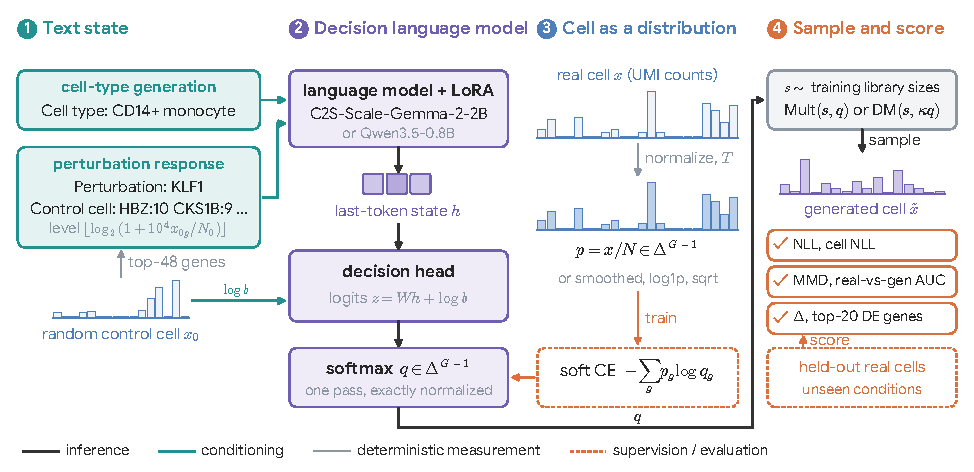
\includegraphics[width=\linewidth]{figs/fig1_method.pdf}
\caption{\textbf{A decision language model reads a text state and returns, in one forward pass, a distribution over a fixed gene panel; every method is scored with the same likelihood and sampler.} (1) The state is a prompt: a cell type, or a perturbation, optionally with a control cell $x_0$. (2) A LoRA-tuned language model encodes the prompt; a linear decision head on the last-token state, with an optional fixed log-prior $b$ (none, the training mean, or the smoothed control cell), gives one logit per gene, and a softmax gives $q$ on the simplex. (3) A real cell is the probability vector $p=x/N$ of its counts; training minimizes the cross-entropy between $p$ and $q$. (4) A shared sampler draws cells from $q$; held-out cells of unseen donors, perturbations or cell types score the model.}
\label{fig:overview}
\end{figure}

The idea is simple, so its value has to be measured, and we organize the paper around three questions.
\textbf{(Q1) Interface.} Does generating the distribution directly beat generating a rank sentence, on the same backbone and budget, and where does the sentence lose?
\textbf{(Q2) Language model.} Does the fine-tuned language model matter, or would any encoder of the condition do?
\textbf{(Q3) Biology.} Does a better gene distribution mean better biology: the downstream response to a perturbation once the trivially induced target gene is set aside, the realism of single cells, and conditions never seen in training?
We answer them on human PBMC (generation for unseen donors and unseen cell types) and on the CRISPRa screen of Norman et al.\ in K562 (response to held-out perturbations), where simple baselines are known to be hard to beat~\citep{ahlmann2025deep,wei2026benchmark}.
Our contributions are:
\begin{enumerate}
\item \textbf{A decision-native generator of single cells.} A softmax decision head over a fixed gene panel turns a fine-tuned language model into a one-pass generator whose output is a normalized gene composition with an exact multinomial score, comparable with count models and simple baselines (Section~\ref{sec:method}).
\item \textbf{A controlled comparison with sentence generation.} On the same backbone and budget, direct decoding gains $0.10$ nats per UMI over autoregressive C2S at $90$ to $540$ times lower decoding cost; rewriting real cells shows that the rank sentence loses most of its likelihood in the map back to counts rather than in the ranks themselves; and matched controls separate the contribution of the language model (Sections~\ref{sec:repr} and~\ref{sec:lm}).
\item \textbf{A biological boundary.} Under leakage-controlled splits, \cad{} matches additive composition of known effects on likelihood and on downstream differentially expressed genes, generates more realistic cells, composes unseen cell types from their names, and fails where no method in our comparison succeeds: genes never perturbed in training (Sections~\ref{sec:pert}--\ref{sec:condgen}).
\end{enumerate}

\section{Background and related work}\label{sec:background}
\paragraph{Decision language models.}
A decision language model returns a probability over a bounded set of options for a typed question in a single pass instead of generating text to be parsed~\citep{typesafe2026jev,deusser2026jev}. The open implementation we build on attaches a classification head to the final hidden state of a pretrained model and trains it with the cross-entropy on soft targets~\citep{unsloth_decision}. The head itself is a softmax classifier; what is new here is the choice of options, the genes of a panel, which makes the answer a cell.

\paragraph{Cells as text and cell foundation models.}
Cell2Sentence fine-tunes language models on rank-ordered gene sentences and has been scaled to billions of parameters~\citep{levine2024cell2sentence,rizvi2025c2sscale}; its case for the representation is that expression is recovered from rank by a log-linear fit with high $R^2$. Other foundation models pretrain on expression tokens (scGPT, Geneformer)~\citep{cui2024scgpt,theodoris2023geneformer}, learn cell embeddings (UCE)~\citep{rosen2023uce}, or decode the whole profile from a bottleneck token (BMFM-RNA)~\citep{danziger2025bmfm}; none returns a normalized distribution from a text condition.

\paragraph{Count generators and perturbation predictors.}
scVI and scANVI decode gene frequencies inside a negative-binomial likelihood conditioned on latent states and labels~\citep{lopez2018scvi,xu2021scanvi}; scDiffusion samples cells with a conditional diffusion model~\citep{luo2024scdiffusion}; the Gene Mover's Distance compares cells as distributions over genes~\citep{gmd2021}. Perturbation predictors such as scGen, CPA, GEARS and State map a perturbation to an expression change~\citep{lotfollahi2019scgen,lotfollahi2023cpa,roohani2024gears,adduri2025state}, and population models learn copulas, flows or transport between control and perturbed cells~\citep{wang2026poppert,yu2026scdfm,chen2026scale,han2026tempobridge,chi2025departures,jiang2026ocoot}. Independent benchmarks find that mean, additive and linear baselines are hard to beat~\citep{ahlmann2025deep,wei2026benchmark} and that control-referenced metrics are inflated by systematic variation~\citep{vinas2025systema}, so our main references are the perturbed mean and additive composition.

\section{Method}\label{sec:method}
\subsection{A cell as a distribution over a fixed panel}\label{sec:why}
Let $x\in\mathbb{N}^G$ be the raw counts of one cell over a fixed panel of $G$ genes, with library size $N=\sum_gx_g$, and let $c$ be a text \emph{state}: a cell type, or a perturbation together with an optional control cell $x_0$. We use $G{=}2048$ genes selected on training cells only (largest dispersion of log-normalized expression among genes detected in more than $1\%$ of training cells; for Norman the training perturbation targets are always included). The panels contain no ribosomal-protein or mitochondrial genes.

\begin{observation}\label{prop:repr}
Let $N>0$ and $p=x/N$. (i) $x\mapsto(N,p)$ is injective, so frequency and library size are lossless; if $x\sim\mathrm{Mult}(N,\pi)$, the log-likelihood of a model $q$ is $N\sum_gp_g\log q_g+\text{const}$, maximized at $q=p$. (ii) A rank sentence (the ordering of genes by $x$) is constant on all count vectors with the same ordering, so it is not injective and keeps no magnitudes. (iii) Log1p or square-root vectors renormalized onto the simplex differ from $p$ unless all nonzero counts are equal, so a model fit to them is not fit to the likelihood of $x$.
\end{observation}
(Proof in Appendix~\ref{app:proofs}.) We distinguish four objects. The decoder outputs $q(c)\in\Delta^{G-1}$, the \emph{composition} of a cell in state $c$: $q_g(c)$ is the probability that a transcript of the cell, drawn at random from its panel UMIs, comes from gene $g$. It is not the probability that $g$ is differentially expressed or that an intervention succeeds. Counts are drawn as $x\mid N,q\sim\mathrm{Mult}(N,q)$. A decoder with a latent variable $z$ outputs $q(c,z)$, and the population of cells in state $c$, $P(x\mid c)$, is then a mixture. A good fit of $q(c)$ to the mean composition does not by itself make $P(x\mid c)$ realistic, so we evaluate both.

\subsection{Decision language model decoder}\label{sec:decoder}
The state is written as a prompt and read by \backbone{}~\citep{c2sgemma_hf,gemma2team2024}, a Gemma-2 model already trained on cell sentences, with rank-16 LoRA adapters on all linear layers~\citep{hu2022lora}. The last-token hidden state $h$ feeds a linear decision head with one logit per panel gene, and $q_\theta(c)=\mathrm{softmax}(Wh+\log b)$, where $\log b$ is an optional fixed log-prior: none, the smoothed training mean, or the smoothed control cell $x_0$, which makes the model a residual on the control cell. The head is initialized at zero, so the model starts as the prior and learns a correction. Training minimizes the cross-entropy $-\sum_gp_g\log q_{\theta,g}(c)$ between the frequency vector $p=x/N$ of a real training cell and the decoded $q_\theta$ (the log1p and square-root targets of Observation~\ref{prop:repr}(iii) are worse on Norman for every metric; Appendix~\ref{app:transform}). For perturbations without a control cell the prompt names the perturbed genes; with a control cell, each training perturbed cell is paired with a random training control cell, and the control cell enters through $\log b$ (Section~\ref{sec:residual}).

\emph{What a categorical state can learn.} When the state is a cell type, the objective averaged over the training cells of the type is minimized, by Gibbs' inequality, at their equal-weight mean frequency; the pooled score below is minimized at the UMI-weighted mean. A decoder conditioned on a label can therefore at best reproduce a type mean (a UMI-weighted loss did not help on validation; Appendix~\ref{app:protocol}).

\subsection{Generation and scoring}\label{sec:likelihood}
A cell is generated by drawing a library size from training cells and counts from $\mathrm{Mult}(s,q)$, or from a Dirichlet-multinomial with a concentration fit on training cells to represent overdispersion; every method uses the same samplers. For a held-out unit (a cell type or perturbation) with cells $x_1,\dots,x_n$, we report $\ell(q)=-\sum_i\sum_gx_{ig}\log q_g/\sum_iN_i$, the multinomial negative log-likelihood (NLL) per UMI up to a model-independent constant; differences between models are exact differences in log-likelihood, and since the score is proper they equal differences in KL divergence to the true mean composition (Appendix~\ref{app:proofs}). Each perturbation receives the same $M=50$ held-out control cells for every method. A model that conditions on a control cell gives one $q_m$ per control cell; its \emph{pooled} NLL uses $\bar q=\frac1M\sum_mq_m$ and its \emph{cell} NLL is the mixture $-\sum_i\log\frac1M\sum_m\exp(\sum_gx_{ig}\log q_{mg})/\sum_iN_i$, which rewards covering the variation between cells. A negative-binomial likelihood with gene-wise dispersions leaves the ordering of methods unchanged (Appendix~\ref{app:nb}). Any method that outputs gene frequencies can be scored this way; methods with a native likelihood (scVI) are additionally scored with their own samples.

\section{Tasks, data and protocol}\label{sec:tasks}
\textbf{Conditional generation.} Human PBMC from Hao et al.~\citep{hao2021seurat4} (CELLxGENE Census; $161{,}159$ cells of 8 donors and 29 cell types): donors P1--P5 train, P6 validation, P7--P8 test; units are cell types with at least 30 held-out cells. \textbf{Perturbation response.} The CRISPRa screen of Norman et al.\ in K562~\citep{norman2019,scperturb2024} ($111{,}445$ cells; 105 single and 131 paired perturbations). In our gene-level split, held-out single genes occur in no training perturbation (an earlier split leaked through training pairs; an audit found it and all its results were discarded). The 76 test perturbations form three strata: 21 unseen single genes, 29 pairs with one unseen gene, and 26 pairs of two genes seen alone in training.

\textbf{Baselines.} The global and cell-type means; the control and perturbed means; \emph{partial additive} composition, in which an unseen gene contributes nothing; additive plus \emph{target induction}, which multiplies each unseen target's frequency by one factor fit on training single perturbations (CRISPRa raises its target about $4.8$-fold), the strongest cheap biology-aware baseline we know; ridge regression; scVI, scANVI and an scGen-style latent shift; GEARS; and autoregressive C2S on the same backbone and budget, whose sentences are mapped to frequencies by the C2S log-rank regression and mixed with the training mean (weight chosen on validation). All baselines are in frequency space and share the sampler.

\textbf{Metrics and statistics.} Besides NLL we report MMD and a real-versus-generated classifier AUC in a PCA space fit on training cells (lower is more realistic), and two biological measures on pseudobulk profiles $\log(1+10^4\bar q)$. Likelihood weights genes by their mass (TMSB4X alone carries about $16\%$ of panel UMIs in K562), so for perturbations we report the \emph{downstream} response: the top-20 differentially expressed genes of each perturbation (largest $|t|$ of a Welch test between its real cells and held-out controls), \emph{after removing the perturbed genes}, and on them $r_{\mathrm{DE}}$, the Pearson correlation of predicted and real change over the control mean, and the fraction of genes changed in the right direction. The perturbed genes are scored separately as \emph{target error}, the absolute error of their predicted log fold change. Units are cell types or perturbations; intervals are paired bootstraps over units. Decisions were made on validation; each test configuration was evaluated once per seed, under promotion rules written down before the test runs; analyses added after the test results are labeled as such (Appendix~\ref{app:protocol}).

\section{Results}\label{sec:results}
\subsection{Q1: one forward pass instead of a sentence}\label{sec:repr}\label{sec:c2s}
\textbf{Same backbone, same budget.} We fine-tuned C2S-Scale-Gemma-2-2B autoregressively on rank sentences with the same LoRA rank, training cells, epochs, batch size and control cells as \cad{}, and decoded its generated sentences with the C2S regression. The sentences are well formed ($115$ genes on average, $99.8\%$ valid names), yet they add no likelihood beyond the perturbed mean ($-0.001$ nats per UMI, CI $-0.006$ to $+0.005$; the validation-chosen mixing weight is the largest on the grid, $0.9$). \cad{} is $0.103$ nats per UMI better (CI $0.071$ to $0.139$) and recovers the downstream response far better ($r_{\mathrm{DE}}$ $0.77$ against $0.56$; Table~\ref{tab:norman_main}). Decoding the same generated sentences with a rank-to-frequency map learned on training cells (described next) barely helps: \cad{} remains $0.098$ nats per UMI better (CI $0.069$ to $0.131$), with the same $r_{\mathrm{DE}}$ gap, so the shortfall lies in the generated sentences and not only in the map that decodes them (post hoc). Decoding costs one forward pass: alone on one A100 at batch size 25, C2S-Gemma needs $1.99$ seconds per generated cell ($530$ new tokens on average), \cad{} $0.004$ seconds per cell with the control cell as a residual and $0.022$ seconds when the control cell is also written as text, $90$ to $540$ times less.

\begin{figure}[t]
\centering
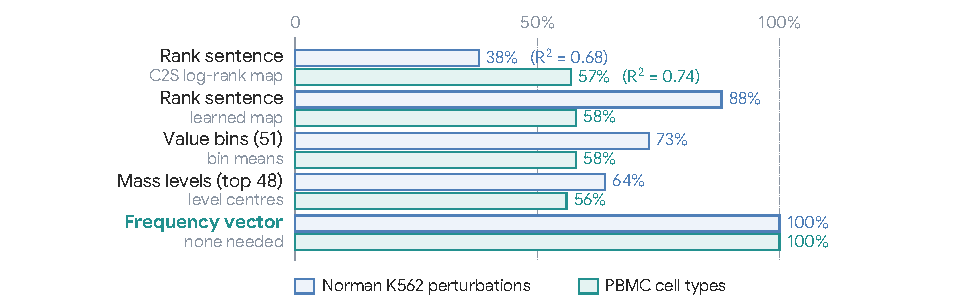
\includegraphics[width=\linewidth]{figs/fig3_representation.pdf}
\caption{\textbf{The likelihood a rank sentence loses depends on how it is decoded.} Real held-out test cells were rewritten in each representation and decoded back to gene frequencies; bars give the share of the likelihood gain of the cells' own frequency vectors over the reference (perturbed mean for Norman, cell-type mean for PBMC) that survives, all estimated from the same cells in the same way. The C2S log-rank map keeps $38\%$ on Norman although it reconstructs log expression with $R^2=0.68$, the criterion used to motivate rank sentences~\citep{levine2024cell2sentence}; a map learned on training cells keeps $88\%$. Ceilings from decoding real cells, not model results; the learned map was added after the test results.}
\label{fig:repr}
\end{figure}

\textbf{Where a sentence loses.} To separate the representation from the model, we rewrote the \emph{real} held-out cells of each unit in a representation, decoded them back to frequencies, and asked how much of the likelihood gain of the cells' own frequency vectors survives (Figure~\ref{fig:repr}). With the published log-rank map, the rank sentence reconstructs log expression well ($R^2=0.68$ on Norman, $0.74$ on PBMC), yet keeps only $38\%$ of the gain on Norman, against $73\%$ for value bins and $64\%$ for mass levels. A map learned on training cells, the mean frequency of each gene at each rank position, keeps $88\%$ from the same sentences ($90\%$ when the library size is also given). Most of the loss is thus in the map from ranks to counts, not in the ranks: the ordering of a K562 cell's genes carries most of its composition, but a sentence has to be decoded, and the decoder decides how much survives; about a tenth is lost under every map we tried. On PBMC the representations do not separate ($56$--$58\%$ each), because cell types differ mostly in which genes are expressed. A generator that outputs the composition needs no such map, and its likelihood is defined by the model itself.

\subsection{Q2: does the language model matter?}\label{sec:lm}\label{sec:backbone}
\autoinput{auto_rev3/tab_e1.tex}
We compared \cad{} without a control cell against two controls, specified before they were run (Table~\ref{tab:e1}), with the same training cells, target, log-prior, softmax output and scoring: the same language model \emph{frozen}, with only an MLP head trained on its last-token state; and a decoder with \emph{no language model}, in which a perturbation is the sum of learned embeddings of its genes (an unseen gene gets a zero embedding) followed by an MLP. On test, the decoder without a language model ties \cad{} in every stratum and for every seed (overall $-0.005$ nats per UMI, CI $-0.017$ to $+0.009$; seeds $1$ and $2$: $-0.007$ and $-0.003$) and on the downstream response ($r_{\mathrm{DE}}$ $-0.012$, CI $-0.042$ to $+0.016$), with $1.1$ million parameters trained in $10$ seconds. The frozen language model is worse ($+0.043$, CI $+0.025$ to $+0.060$; $r_{\mathrm{DE}}$ $-0.108$), most on pairs of seen genes ($+0.096$). On validation the no-language-model decoder was $0.013$ nats worse (CI $0.000$ to $0.028$), so the pre-registered rule applies: the likelihood gain over C2S and the perturbed mean comes from decoding the distribution directly, not from knowledge in the language model. Fine-tuning is what makes the language model as good a decoder of the condition as a purpose-built encoder; what the language model adds is the interface, one prompt format for any state, which is what lets the same model generate cell types it has never seen (Section~\ref{sec:condgen}). Two results point to what the language model contributes. Replacing gene symbols by opaque identifiers in the prompt worsens the downstream response even on pairs of seen genes ($r_{\mathrm{DE}}$ $0.87$ against $0.89$, overall $0.69$ against $0.77$), so names help the model organize what it learns from training perturbations; but on unseen single genes the names bring nothing measurable ($+0.007$ nats, CI $-0.022$ to $+0.030$), nor do NCBI gene summaries (validation). The backbone matters modestly: across three seeds the C2S-initialized Gemma is $0.011$ to $0.012$ nats better than the general-purpose Qwen3.5-0.8B on both tasks, more than the seed spread ($0.001$ to $0.003$), without changing any ranking; LoRA ranks 8 to 64 give the same NLL.

\subsection{Q3a: perturbation biology}\label{sec:pert}
\autoinput{auto_rev3/tab_norman_main.tex}
\textbf{Likelihood and realism (Table~\ref{tab:norman_main}).} Without a control cell, \cad{} is $0.104$ nats per UMI better than the perturbed mean (CI $0.071$ to $0.139$) and ties the additive baseline ($-0.009$, CI $-0.037$ to $+0.010$). Its generated cells are closer to real ones than additive cells (MMD $0.039$ against $0.052$; AUC $0.81$ against $0.86$), but not than those of the scGen-style shift, which moves each control cell individually. GEARS with default settings is $0.47$ nats above the perturbed mean after its regression output is mapped to frequencies (Appendix~\ref{app:val}); this measures that conversion as much as the model.

\autoinput{auto_rev3/tab_strata.tex}
\textbf{Downstream response, target gene set aside (Table~\ref{tab:strata}; post hoc).} CRISPRa raises its own target, so a model can look right on the target alone. With the perturbed genes removed, \cad{} reproduces the direction of $89\%$ of the top-20 downstream genes and ties additive on $r_{\mathrm{DE}}$ overall ($0.77$ against $0.77$; $+0.004$, CI $-0.033$ to $+0.040$) and in every stratum, and is better than scGen-style ($0.72$) and C2S ($0.56$). On the target genes themselves it is \emph{worse} than additive on pairs (target error $0.51$ against $0.27$ with one unseen gene, $0.58$ against $0.39$ with both seen). The error has a direction: the real induction of a target is about $1.7$ log units, additive composition copies it from the training single perturbation almost without bias ($+0.04$ to $+0.09$), and \cad{} under-predicts it by about $0.5$, shrinking a large gene-specific change toward the mean composition it learns a correction to (only $4$ of the $21$ unseen single targets are in the panel, so this concerns pairs). Adding target induction to the additive baseline lowers its target error further but changes its NLL by at most $0.003$ nats, because a target gene carries little transcript mass; likelihood and target accuracy are separate properties and we report both.

\textbf{Unseen genes.} On the $21$ genes never perturbed in training no method in our comparison does well: \cad{} ties the perturbed mean ($-0.006$, CI $-0.025$ to $+0.018$; $r_{\mathrm{DE}}$ $0.54$ against $0.51$), while a split-half oracle lies $0.108$ nats below it (Appendix~\ref{app:kfold}). For the median unseen gene, MAML2, its own induction is the largest change among its top-20 DE genes (Figure~\ref{fig:demo}b); a decoder that has never seen the gene perturbed cannot infer this from its name.

\subsection{Q3b: per-cell variation}\label{sec:residual}\label{sec:heads}
A single $q$ per perturbation leaves all cell-to-cell variation to the sampler. With the control cell as the log-prior ($b=\mathrm{smooth}(x_0)$, not written in the prompt), the cell NLL improves from $5.186$ to $5.129$ and the cells become more realistic (MMD $0.030$, AUC $0.79$), approaching scGen-style on MMD. Writing the control cell into the prompt instead loses this gain ($+0.019$ nats per cell, CI $+0.012$ to $+0.027$). A version of the residual without a language model, in which the additive shift replaces the learned correction, reaches the same likelihood ($5.134$) but less realistic cells (MMD $+0.008$, AUC $+0.030$ relative to \cad{}). The residual has a cost: its downstream $r_{\mathrm{DE}}$ falls to $0.72$, below additive ($-0.046$, CI $-0.092$ to $-0.008$), because each control cell's own deviations enter the prediction. Two heads keep the single pass and the normalization of $q$ while modeling variation the flat softmax lacks (Appendix~\ref{app:heads}): a low-rank logistic-normal head, $q(c,z)$ along $16$ learned gene programs, lowers the cell NLL to $5.096$ without any control cell at the cost of the pooled NLL ($+0.062$); a negative-binomial head with per-gene dispersion improves the change correlation over all genes ($r_\Delta$ $+0.020$) at a small cost in NLL. Gene--gene correlations of generated cells on 100 variable genes are close to those of real cells for every method at this sequencing depth (Appendix~\ref{app:coexpr}).

\subsection{Q3c: cell types, known and unseen}\label{sec:condgen}
\autoinput{auto_rev3/tab_pbmc.tex}
\textbf{Known types (Table~\ref{tab:pbmc_main}).} As the remark of Section~\ref{sec:decoder} predicts, no model improves on the cell-type mean in likelihood on unseen donors: \cad{} is slightly worse ($+0.017$, CI $+0.001$ to $+0.036$), scVI and scANVI tie it, and on validation \cad{} gives the same NLL to four decimals for every LoRA rank and both backbones. Sample realism is decided by the source of cell-to-cell variation: scVI sampling from its own negative binomial reaches the lowest MMD and AUC ($0.92$), every frequency decoder relies on the shared sampler, and no generator is near indistinguishable from real cells of unseen donors (AUC $\ge0.92$).

\autoinput{auto_rev3/tab_zeroshot.tex}
\textbf{Unseen types (Table~\ref{tab:zeroshot}).} A model indexed by cell type cannot generate a type it has never seen; a decoder that reads the type's name can. In five leave-types-out folds over $19$ types, \cad{} generates each held-out type from its name and Cell Ontology definition. It is $0.707$ nats per UMI better than the global mean (CI $0.545$ to $0.862$) and better than the nearest Cell Ontology type and the pooled Cell Ontology parents; it ties a string-matching baseline that copies the training type whose name shares the most words ($-0.058$, CI $-0.219$ to $+0.101$) but recovers the requested type far more often ($0.14$ against $0.02$). The definition adds nothing beyond the name, and opaque identifiers remove the gain: \cad{} generalizes by composing the words of type names, and we find no evidence that it uses knowledge beyond them.

\section{Discussion}
Letting a decision language model answer with a gene distribution makes a language model a single-cell generator whose output is a cell's composition rather than a sentence about it. The interface has concrete consequences: generation costs one forward pass, the model's likelihood is defined without a reconstruction map, and every method can be compared on one proper score. The comparison with rank sentences shows why the last point matters: the same sentences keep $38\%$ or $88\%$ of the achievable likelihood depending on the map chosen to decode them, so a sentence model's quality cannot be separated from a post hoc choice, whereas a distribution is scored as produced. Our controls are equally clear about what the language model does not do: a decoder of learned gene embeddings with the same output matches it on perturbations of known genes, so the decision-native output, not language-model knowledge, carries the gain; the language model makes the interface general, from perturbation names to cell-type names and definitions, and that generality is what enables generation of unseen cell types.

A better gene distribution is not yet better biology, and our biological results draw a clear boundary. Where training contains the perturbed genes, the decoder matches additive composition on likelihood and on the downstream program, and generates more realistic cells; it is worse on the size of the target's own induction; and it does not transfer to genes it has never seen perturbed, where neither its names nor gene descriptions help. A categorical cell type caps any decoder at the type mean, while names let it compose unseen types. The output $q$ is a composition, not a probability of differential expression or of an intervention's success; a decision head trained on such events, with calibration measured on held-out perturbations, is the natural next step for the decision-native interface, together with richer states (donor, cell and pathway context) and heads that model dispersion and covariance jointly.

\paragraph{Limitations.}
One dataset per task, a $2048$-gene panel and CRISPRa only; held-out control cells are not paired with perturbed cells, so cell NLL rewards covering cell states rather than predicting a counterfactual; GEARS was run with default settings and CPA and the transport and flow models were not compared, because they do not output a distribution over a fixed gene list; zero-shot types were evaluated with the Qwen backbone; the downstream, target, co-expression and learned-rank-map analyses were added after the test results (Appendix~\ref{app:protocol}).

\paragraph{Code availability.} Code, held-out unit lists, run scripts and table-generation scripts are available with a README at \url{https://anonymous.4open.science/r/CellAsDistribution-R27}.
\paragraph{AI use statement.} Code, experiments, tables, figures and a first draft of this text were produced with assistance from Claude (Anthropic); the authors reviewed all content and are responsible for it.

\bibliographystyle{unsrtnat}
\bibliography{refs}
\clearpage
\appendix
\begin{center}{\large\bfseries Supplementary material}\\[2pt]\cad: Decision-Native Language Modeling of Single-Cell Gene Composition\end{center}
\suppressfloats[t]
\section{K-fold analysis on Norman}\label{app:kfold}
This analysis was run with the Qwen3.5-0.8B backbone (\cadf{}, the flat decoder of the population-level analysis) before the Gemma backbone was added.
\autoinput{auto/norman_kfold_table.tex}
\begin{figure}[t]
\centering
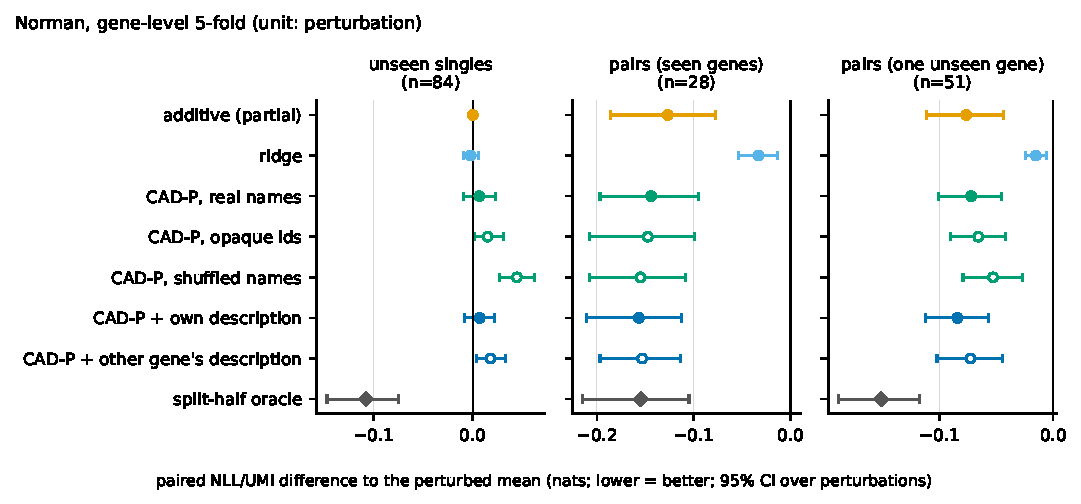
\includegraphics[width=\linewidth]{figs/fig_kfold_forest.pdf}
\caption{Gene-level 5-fold on Norman, population level: paired held-out NLL difference to the perturbed mean (bars: 95\% bootstrap over perturbations; hollow: identity or knowledge controls; diamond: split-half oracle).}
\label{fig:forest}
\end{figure}
Pooled over five gene-level folds, the flat decoder ties the partial-additive baseline on pairs of seen genes ($-0.017$, CI $-0.060$ to $+0.021$, $n=28$) and on pairs with one unseen gene ($+0.004$, CI $-0.014$ to $+0.022$, $n=51$), and it beats ridge.
The split-half oracle lies $0.108$ nats below the perturbed mean on unseen single genes, so headroom exists; descriptions and shuffled names do not help, and shuffled names are harmful ($+0.045$).
A one-parameter target-induction baseline, which raises the unseen target gene's frequency, is better than every learned decoder on the $75$ genes whose target is in the panel ($-0.013$, CI $-0.031$ to $-0.004$).
On the test split, \cadf{} (Qwen backbone) is $0.097$ better than the perturbed mean and ties additive ($-0.003$, CI $-0.031$ to $+0.019$).

\section{Training details}\label{app:train}
Table~\ref{tab:train} lists the training settings of the decision language models, and the paragraphs below it describe the scVI-based baselines.

\begin{table}[h]
\centering
\scriptsize
\begin{tabular}{@{}p{0.22\linewidth}p{0.74\linewidth}@{}}
\toprule
Setting & Value \\
\midrule
Optimizer, schedule & AdamW (weight decay $0$), one-cycle schedule with $5\%$ warm-up, gradient clipping at $1.0$ \\
Learning rates & $2\times10^{-4}$ (LoRA adapters), $10^{-3}$ (decision head, zero-initialized) \\
Batch size, budget & $16$; one epoch over $20{,}000$ training cells drawn at random ($1{,}250$ steps) \\
LoRA & rank $16$, $\alpha=16$, dropout $0$, all linear layers; rank $8$ and $64$ for the sensitivity run \\
Precision, attention & bf16; eager attention and gradient checkpointing for Gemma-2 \\
Output vocabulary & the $2048$ panel genes as classes; no new tokens, gene names are tokenized as plain text \\
Control-cell text & $48$ most abundant genes with $14$ log-mass levels; $200$ gene names for the rank variant \\
Seeds & test: Gemma and Qwen $0,1,2$; validation: Gemma $3407$ (default), $1$, $2$; Qwen $1,2$; variants of Appendix~\ref{app:protocol}: Qwen seed $0$ (the seed changes the sampled training cells and the sampler) \\
Negative-binomial head & inverse dispersion $\log\theta_g(c)=\beta_g+v_g^\top h$, initialized at $\theta=1$ and clipped to $[e^{-6},e^{8}]$; loss: negative-binomial NLL of the raw panel counts with mean $N_iq_g$, per UMI \\
Low-rank head & $k=16$ programs; amplitude $a(h)=\mathrm{softplus}(\cdot)$ initialized at $1$; encoder of the target cell: $\log(1+10^4x/N)\to256$ (GELU) $\to2k$; one reparameterized sample per cell; KL weight raised linearly from $0$ to $1$ over the first $30\%$ of steps \\
C2S-Gemma baseline & C2S-Scale-Gemma-2-2B, LoRA $r=16$ on all linear layers, lr $2\times10^{-4}$, one-cycle schedule, $20{,}000$ cells, one epoch, batch $16$ (micro-batches of $2$); control and target as top-200 rank sentences; loss on the response only; sampling with top-$k$ $50$, top-$p$ $0.95$, up to $1024$ new tokens \\
Evaluation & $M=50$ held-out control cells per perturbation, the same for every method (earlier runs: drawn separately per method); $300$ generated cells per unit \\
Hardware, time & one A100 40\,GB; run alone, Qwen takes $6$ to $8.5$ min and Gemma $9.5$ to $24$ min per run ($90$ to $100$ min with the 200-gene rank text; wall-clock was longer when jobs shared the GPU); Gemma peak memory $8.7$\,GB \\
\bottomrule
\end{tabular}
\caption{Training settings of the decision language models.}
\label{tab:train}
\end{table}

\paragraph{scVI and scANVI.}
Both are trained on training cells of the panel with a negative-binomial likelihood, $30$ latent dimensions and $60$ epochs (scANVI: $15$ further epochs with cell-type labels).
The frequency vector of a cell type is the mean decoder output over up to $3000$ training cells of that type.

\paragraph{scGen-style baseline.}
An scVI model is trained on all training cells.
The latent shift of a single gene is the mean latent state of its perturbed cells minus that of the control cells, the shift of a pair is the sum of the shifts of its known genes, and a perturbation with no known gene uses the mean shift of all training perturbations.
Each held-out control cell is encoded, shifted and decoded with library size one.

\section{Negative-binomial evaluation}\label{app:nb}
For a held-out cell $i$ of a unit with library size $s_i$ and model frequency $q$, the count of gene $g$ is scored as $\mathrm{NB}(x_{ig}\mid\mu=s_iq_g,\phi_g)$ with variance $\mu+\phi_g\mu^2$.
The dispersions $\phi_g$ come from a method-of-moments fit on library-normalized training counts with the within-unit variance pooled over units (median $\phi=26.5$ for PBMC and $9.0$ for Norman, clipped to $[10^{-3},10^2]$).
The score is the negative log-likelihood per UMI, which is on a different scale from the multinomial score because it includes the zeros, so only differences are compared (Table~\ref{tab:nb}).
It uses the pooled frequency of a unit, so it does not reward conditioning on a control cell.

\begin{table}[h]
\centering
\scriptsize
\begin{tabular}{llrr}
\toprule
Task & Model & $\Delta$NB [95\% CI] & $\Delta$multinomial \\
\midrule
PBMC (vs.\ cell-type mean) & global mean & $+0.302$ [$+0.252$, $+0.352$] & $+1.125$ \\
 & scVI & $+0.004$ [$+0.001$, $+0.007$] & $+0.005$ \\
 & scANVI & $+0.002$ [$+0.000$, $+0.005$] & $+0.004$ \\
 & \cadc{} (Gemma) & $+0.004$ [$+0.002$, $+0.006$] & $+0.017$ \\
 & \cadc{} (Qwen) & $+0.005$ [$+0.002$, $+0.009$] & $+0.030$ \\
\midrule
Norman (vs.\ perturbed mean) & additive & $-0.014$ [$-0.023$, $-0.004$] & $-0.094$ \\
 & ridge & $-0.008$ [$-0.010$, $-0.006$] & $-0.024$ \\
 & scGen-style & $-0.014$ [$-0.021$, $-0.008$] & $-0.085$ \\
 & \cadc{} (Gemma, no control) & $-0.021$ [$-0.027$, $-0.015$] & $-0.104$ \\
 & \cadc{} (Gemma, control) & $-0.017$ [$-0.023$, $-0.012$] & $-0.091$ \\
 & \cadc{} (Qwen, no control) & $-0.019$ [$-0.025$, $-0.013$] & $-0.092$ \\
 & \cadc{} (Qwen, control) & $-0.015$ [$-0.020$, $-0.010$] & $-0.078$ \\
\bottomrule
\end{tabular}
\caption{Negative-binomial and multinomial NLL per UMI relative to the reference (test split, seed 0; earlier runs, with control cells not matched across methods; negative favors the model; paired bootstrap over cell types or perturbations).}
\label{tab:nb}
\end{table}

On PBMC the negative-binomial score separates the decoders slightly more than the multinomial score does: \cadc{} is reliably, but marginally ($0.004$ nats), worse than the cell-type mean.
On Norman the ordering of the methods is the same as under the multinomial score.

\section{Worked examples: prompts and decoded distributions}\label{app:demo}
Figures~\ref{fig:demo} and~\ref{fig:demo2} show, for every use case, the exact prompt that the decision language model reads and the distribution it returns, next to the held-out ground truth.
The examples are not hand-picked.
In each case, the shown unit is the held-out cell type or perturbation whose paired NLL difference between \cad{} and the case's reference is the median over the units of that case, so half of the units look better and half look worse.
The cases are:
\begin{itemize}
\item conditional generation on unseen PBMC donors, against the cell-type mean;
\item perturbation response without a control cell, one example per stratum of the gene-level split (unseen single gene, pair with one unseen gene, pair of two seen genes), against the additive baseline;
\item perturbation response with a control cell, for a pair of two seen genes, once with the control cell both written as mass-level text in the prompt and used as the residual prior (the prompt shows a real serialized control cell), and once with the control cell used only as the residual prior;
\item zero-shot cell types (fold 0, so the median of its $4$ held-out types), against the mean of the nearest training type in the Cell Ontology.
\end{itemize}
The ground truth is the pooled frequency of all held-out real cells of the unit.
For a control-cell model the plotted distribution is the mean over the $M=50$ matched control cells, and the prompt shown is the one built from the first of them.
For perturbations, the right panel compares the log fold change over the held-out control mean on the unit's top-20 differentially expressed genes (largest $|t|$ of a Welch test between its real cells and the held-out control cells, computed on real cells only).
The selected units and the numbers quoted for them are:
\autoinput{figs/demo_outputs_text.tex}

\begin{figure}[p]
\centering
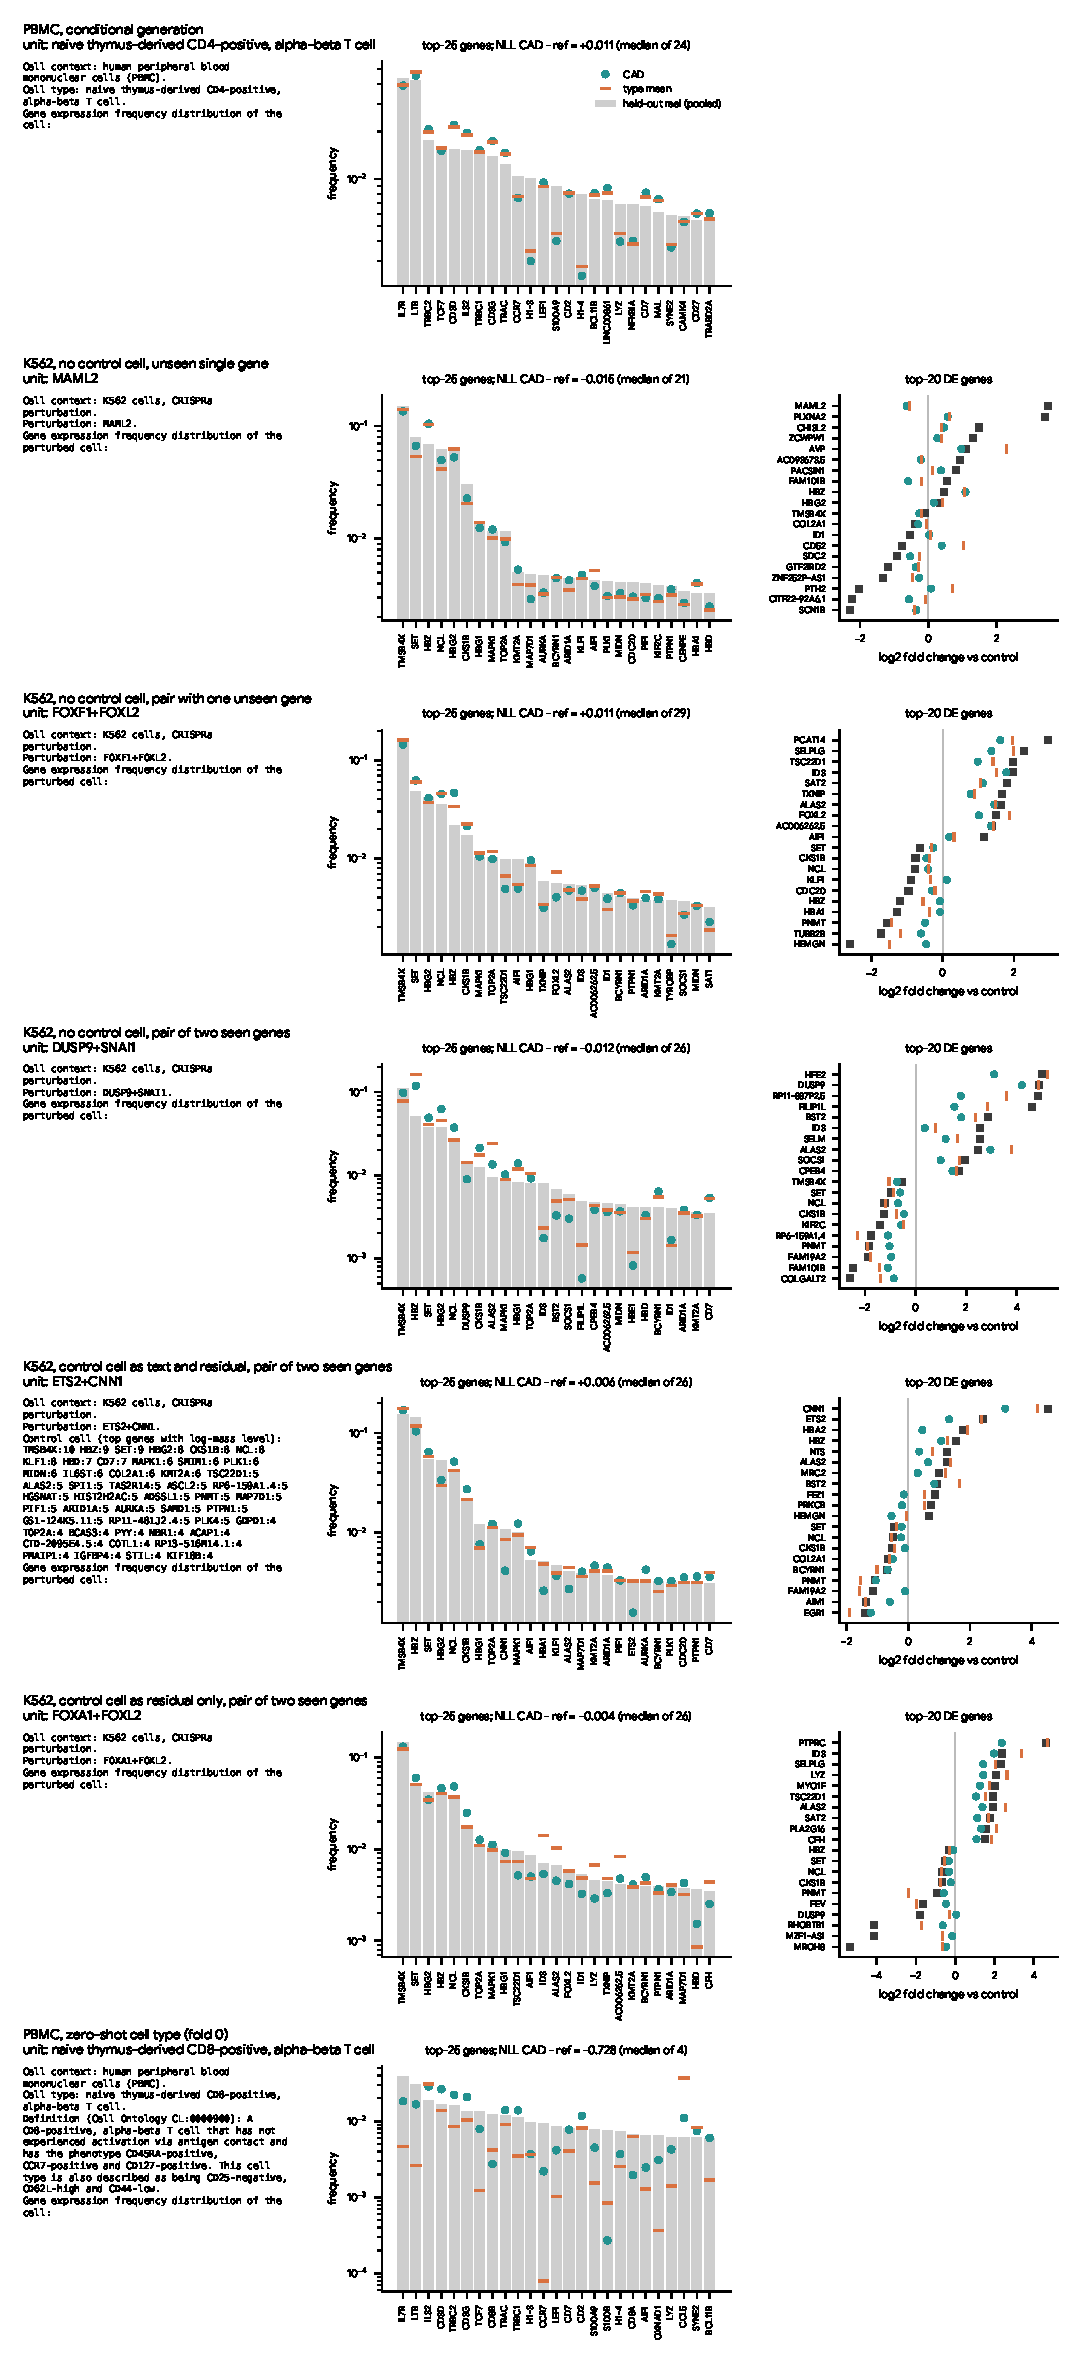
\includegraphics[width=0.94\linewidth,trim=0 484 0 0,clip]{figs/demo_outputs.pdf}
\caption{Prompts and decoded distributions, one median example per use case (test split). Left: the prompt given to \cad{}. Middle: frequency of the 25 genes with the highest ground-truth frequency (log scale) for the held-out real cells (grey bars), \cad{} (teal dots) and the reference (orange ticks). Right, perturbations only: log fold change over the held-out control mean on the unit's top-20 DE genes for real cells, \cad{} and the reference. Shown here: conditional generation and the three strata without a control cell; the remaining cases are in Figure~\ref{fig:demo2}.}
\label{fig:demo}
\end{figure}
\begin{figure}[p]
\centering
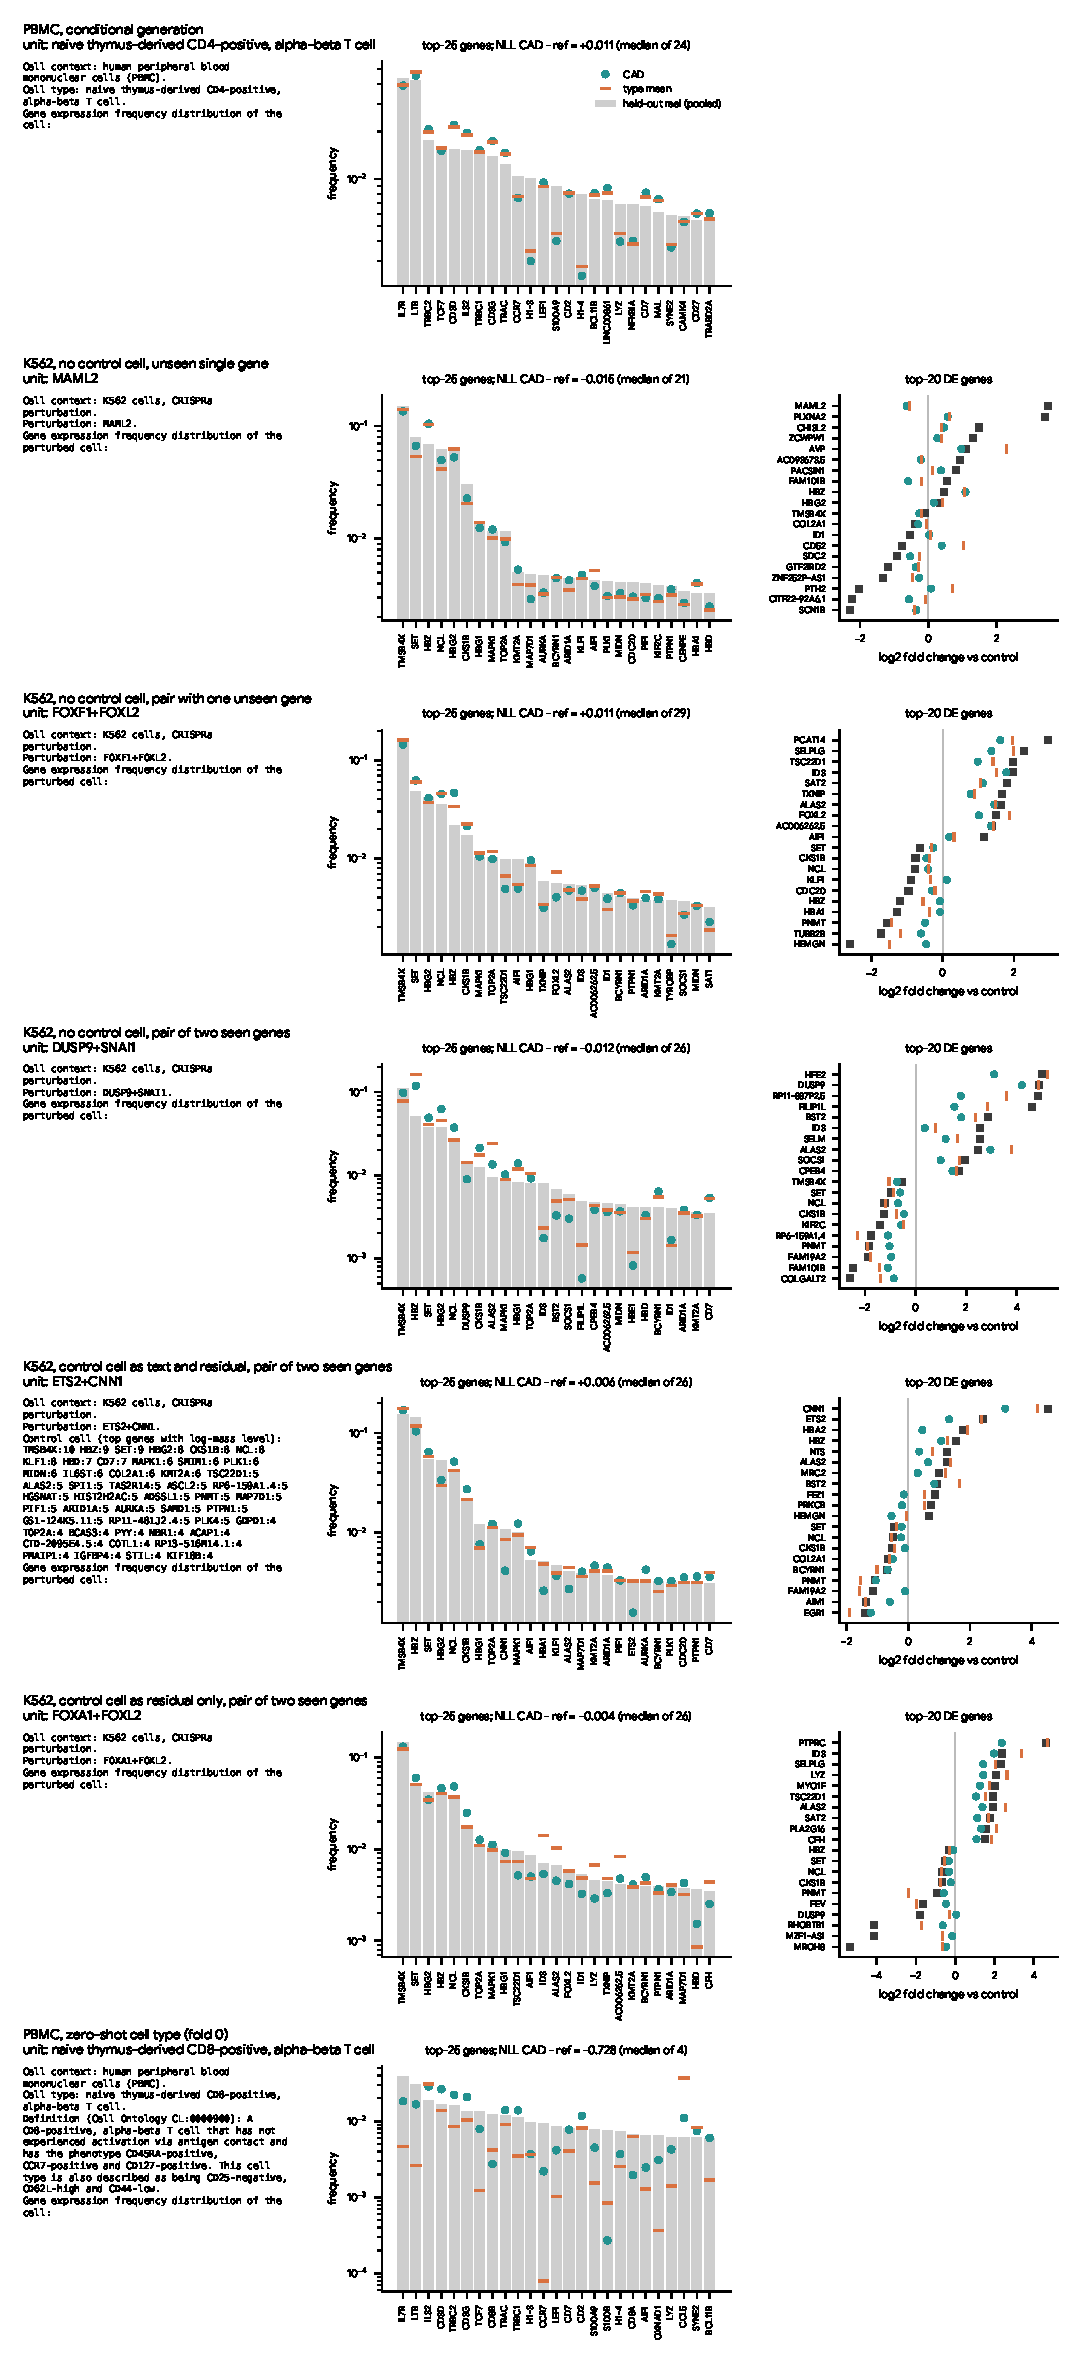
\includegraphics[width=0.94\linewidth,trim=0 0 0 650,clip]{figs/demo_outputs.pdf}
\caption{Prompts and decoded distributions (continued from Figure~\ref{fig:demo}): perturbation response with the control cell as text and residual, and as residual only, and zero-shot cell types.}
\label{fig:demo2}
\end{figure}

\section{Target transformations}\label{app:transform}
\autoinput{auto/pbmc_val_transform_table.tex}
Table~\ref{tab:pbmc_val_transform} (validation, $19$ cell types, Qwen3.5-0.8B backbone) shows that the transformation trades likelihood for sample quality on PBMC.
Frequency gives the best NLL, and smoothing is worse on every metric ($+0.172$ nats, 95\% CI $+0.144$ to $+0.196$; MMD $+0.074$).
Log1p and square-root targets are $+0.144$ and $+0.118$ nats worse in NLL, yet their MMD is lower ($-0.057$, CI $-0.107$ to $-0.016$, and $-0.057$, CI $-0.109$ to $-0.014$) with unchanged real-versus-generated AUC.
A flatter target moves mass to rarely expressed genes, which lowers the likelihood of raw counts while placing generated cells closer to real ones in PCA space.

For perturbation response the trade-off does not appear (Gemma backbone, test, $76$ perturbations; Appendix~\ref{app:val}).
Relative to the frequency target, log1p is $0.288$ nats worse in NLL (CI $+0.249$ to $+0.333$) and square root $0.250$ worse (CI $+0.219$ to $+0.282$), and both also have a higher MMD ($0.094$ and $0.087$ against $0.039$) and a higher real-versus-generated AUC ($0.875$ and $0.871$ against $0.811$).
We therefore keep frequency as the default, and we report the sample-quality advantage of flattened targets as specific to the conditional PBMC task in our experiments.


\section{UMAP views of generated cells}\label{app:umap}
\begin{figure}[t]
\centering
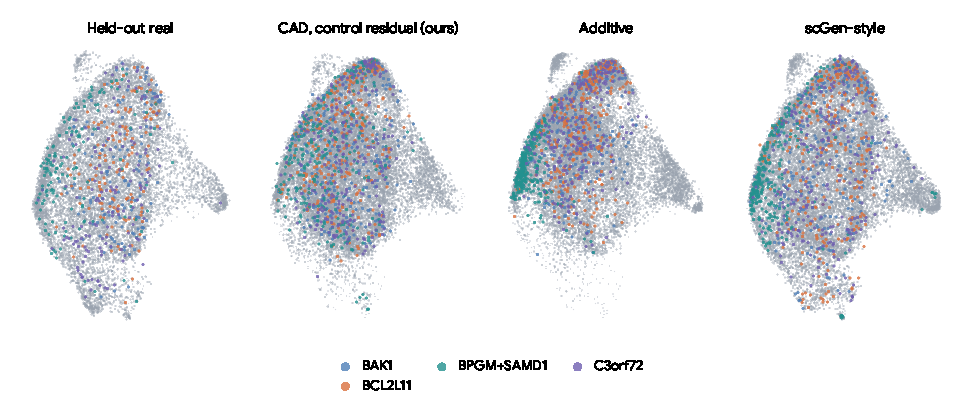
\includegraphics[width=\linewidth]{figs/umap_pert_rev2.pdf}
\caption{UMAP of held-out real perturbed K562 cells (test split) and of cells generated from the matched control cells by \cad{} with the control-cell residual (Gemma, seed 0), by the additive baseline and by the scGen-style latent shift, all drawn with the shared multinomial sampler. PCA and UMAP are fit on real cells only, and generated cells are projected. Colors: the four most frequent held-out perturbations; grey: the others.}
\label{fig:umap-pert}
\end{figure}
\begin{figure}[t]
\centering
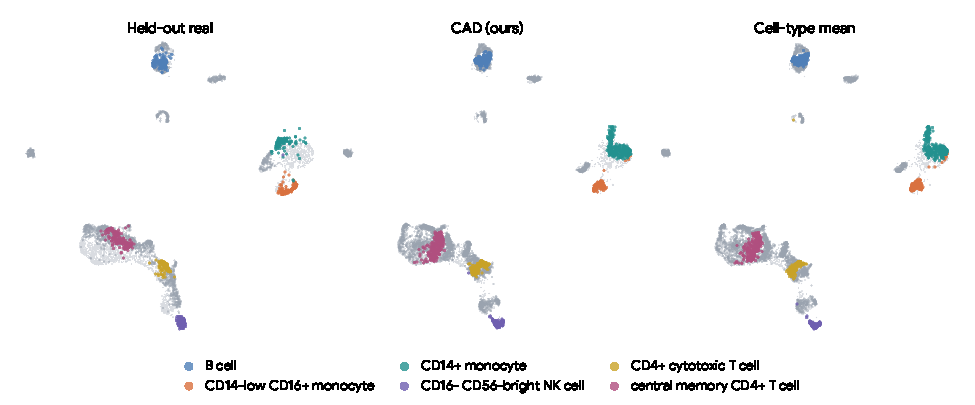
\includegraphics[width=\linewidth]{figs/umap_cond_rev2.pdf}
\caption{UMAP of held-out real PBMC cells (unseen donors, test split) and of cells generated by \cad{} (Gemma, seed 0) and by the cell-type mean with the same sampler. PCA and UMAP are fit on real cells only, and generated cells are projected. Colors: the six most frequent cell types; grey: the others.}
\label{fig:umap-cond}
\end{figure}

\section{Decision rules and the test-split record}\label{app:protocol}
Beyond the main configurations, every variant was first run on validation (Qwen3.5-0.8B backbone, seed~0, matched control cells, comparators re-run with the same control cells) and promoted to the test split only if, on validation, its paired 95\% interval against its comparator excluded zero in its favor on at least one metric fixed in advance, and no such metric was worse with an interval excluding zero; at most three new configurations were promoted. Promoted configurations were then run once per seed (0, 1, 2) on test with the Gemma backbone. The rules and decisions were written to the repository before the test runs.

\begin{table}[h]
\centering
\scriptsize
\setlength{\tabcolsep}{3pt}
\begin{tabular}{p{0.30\linewidth}p{0.22\linewidth}p{0.24\linewidth}p{0.16\linewidth}}
\toprule
Variant & Comparator & Primary metric(s) & Decision \\
\midrule
Control residual, no control text & control residual with mass text & per-cell NLL & beat comparator; test, 3 seeds \\
Control text, no residual & control residual with mass text & per-cell NLL & worse; test, 1 seed (ablation) \\
Contrast control text & control residual with mass text & per-cell NLL, MMD, $r_\Delta$ & promoted \\
Gene summaries in the prompt & other gene's summary; opaque ids & NLL, $r_\Delta$ on unseen singles & not promoted \\
UMI-weighted loss & same model, equal weights & NLL, $r_\Delta$, $r_{\mathrm{DE}}$ & not promoted \\
Negative-binomial head & softmax head & NLL, $r_\Delta$, $r_{\mathrm{DE}}$ & promoted (Norman only) \\
Low-rank head & softmax head & per-cell NLL, MMD, AUC & promoted (no control cell) \\
Zero-shot cell types & nearest Cell Ontology type & NLL & passed (gate G3) \\
C2S-Gemma mixing weight & --- & validation NLL & $0.9$ (grid maximum) \\
\bottomrule
\end{tabular}
\caption{Validation decisions taken before the test runs.}
\label{tab:decisions}
\end{table}

Four analyses were added after the test results had been seen, and are labeled as such where they appear: the $R^2$ of the rank reconstruction (Section~\ref{sec:repr}), the control-cell residual without a language model (Section~\ref{sec:residual}; a first version that divided by the pooled control frequency instead of the mean prior was not a fair analogue and was discarded), the name-overlap and Cell Ontology parent baselines for zero-shot types (Section~\ref{sec:condgen}), and the decoding-speed benchmark (Section~\ref{sec:backbone}). Each can only weaken our claims.

Deviations, all disclosed: a $128$-gene mass-level control text was not evaluated because it repeatedly ran out of GPU memory; three Qwen control-residual test runs ran out of memory during the test lanes and were re-run alone with the same configuration; and the zero-shot gate was applied on the $8$ types of folds 0 and 1 because three validation runs of folds 2--4 had run out of memory, which were then re-run (on all $19$ types the gate gives the same decision, $-0.476$ nats per UMI, CI $-0.971$ to $-0.123$).

\paragraph{Revision 3 (written before its new runs).} Two controls for the language model (a frozen backbone with an MLP head, and a decoder without a language model; Section~\ref{sec:lm}) were specified, with their comparators, metrics and decision rule, in \texttt{experiments/PREREGISTRATION\_rev3.md} before they were run. As controls rather than candidate improvements, they were run on validation (Qwen, seed 0) and then on test (Gemma, seeds 0--2) whatever their validation result. Four further analyses of saved outputs were added after the test results had been seen: the downstream and target metrics with the perturbed genes excluded and the additive-plus-target-induction baseline (Section~\ref{sec:pert}); the learned rank-to-frequency maps, including the re-decoding of the C2S-Gemma sentences (Section~\ref{sec:repr}); and the co-expression comparison (Appendix~\ref{app:coexpr}). They use no new training on test data. Without exclusion, the downstream code reproduces the earlier $r_{\mathrm{DE}}$ values exactly.

\section{Distributional heads}\label{app:heads}
\textbf{Negative-binomial head.} The head adds a per-gene inverse dispersion $\theta_g(c)$, $\log\theta_g(c)=\beta_g+v_g^\top h$, and is trained on the negative-binomial likelihood of the counts with mean $N_iq_g$, so high-mass genes no longer dominate the gradient. On the Norman test split (no control cell, against the softmax head) it raises $r_\Delta$ by $0.020$ (CI $0.012$ to $0.029$), and by $0.049$ on unseen single genes (CI $0.034$ to $0.067$), at a small cost in pooled multinomial NLL ($+0.015$, CI $+0.006$ to $+0.028$). On PBMC it did not help on validation and was not promoted.

\textbf{Low-rank logistic-normal head.} The logits become $z=Wh+\log b+U\,\mathrm{diag}(a(h))\,\epsilon$ with $\epsilon\sim\mathcal N(0,I_{16})$, so $q(c,z)$ varies from cell to cell along $16$ learned gene programs; training uses a variational bound with an encoder of the target cell, and generation draws $\epsilon$ from the prior. Without a control cell it lowers the cell NLL by $0.089$ (CI $0.080$ to $0.098$) on Norman, reaching the scGen-style model ($-0.009$, CI $-0.019$ to $+0.002$), and on PBMC from $5.623$ to $5.552$. The pooled NLL of the mean over draws is worse ($+0.062$, CI $+0.040$ to $+0.087$) and $r_\Delta$ lower ($-0.067$). The cell NLL is estimated from $50$ (Norman) or $300$ (PBMC) prior draws; this log-mean-exp estimator is biased upwards.

\section{Co-expression of generated cells}\label{app:coexpr}
\autoinput{auto_rev3/tab_coexpr.tex}
For each test perturbation with at least $100$ real cells, on the $100$ panel genes with the largest variance of log-normalized expression in training cells, we compared the gene--gene Pearson correlations across real cells with those across the method's generated cells (multinomial sampler), and the total variance and the share of variance on the first principal component (Table~\ref{tab:coexpr}; post hoc). With a median of about $216$ panel UMIs per cell, correlations are dominated by counting noise, and every generator is within $0.005$ of the others in correlation error. Resampling real cells of training perturbations is further from the held-out cells ($0.093$), so the generated cells reproduce perturbation-specific co-variation at least as well as real cells of other conditions. The low-rank head and the scGen-style shift, which model variation between cells explicitly, are slightly closer than the flat decoders, and the additive baseline under-disperses (variance ratio $0.94$).

\section{Additional tables}\label{app:val}
\autoinput{auto_rev3/tab_norman_full.tex}
The tables in this section and in Appendix~\ref{app:transform} come from the earlier runs, in which the control cells were drawn separately for each method; the main-text tables use matched control cells.
Table~\ref{tab:norman_test_transform} (test) compares the target transformations for perturbation response with the Gemma backbone, and Table~\ref{tab:norman_test_rank_vs_mass} (test) compares the two control-cell formats.
Tables~\ref{tab:val_cond} and~\ref{tab:val_pert} repeat the comparison with the other generators on the validation split, on which all decisions were made; Table~\ref{tab:val_pert_lora} shows the LoRA-rank sensitivity on Norman (validation).
\autoinput{auto_test/norman_test_transform_table.tex}
\autoinput{auto_test/norman_test_rank_vs_mass_table.tex}
\autoinput{auto_rev/val_cond_table.tex}
\autoinput{auto_rev/val_pert_table.tex}
\autoinput{auto_test/val_pert_lora_table.tex}

\section{Proofs}\label{app:proofs}
\textbf{Observation~\ref{prop:repr}.} (i) $x=Np$ recovers the counts from $(N,p)$, and $(N,p)$ is a function of $x$. Under $\mathrm{Mult}(N,q)$, $\log P(x)=\log\frac{N!}{\prod_gx_g!}+\sum_gx_g\log q_g=\text{const}+N\sum_gp_g\log q_g$, which by Gibbs' inequality is maximized over $q\in\Delta$ at $q=p$. (ii) For any $x$ with at least two distinct nonzero counts, $x$ and $2x$ have the same ordering and hence the same sentence, and so do $x$ and any count vector obtained by a strictly increasing change of the counts. (iii) $x$ and $2x$ have the same binarization. For $f(t)=\log(1+t)$ or $f(t)=\sqrt t$, the renormalized vector is $p'_g=f(x_g)/\sum_hf(x_h)$, and $p'=p$ requires $f(x_g)/x_g$ to be equal for all genes with $x_g>0$; because $f(t)/t$ is strictly decreasing for $t>0$, this holds only when all nonzero counts are equal.

Throughout, $\Delta$ is the simplex over the $G$ panel genes and modules $S_1,\dots,S_M$ partition the genes; P1, P3 and P4 concern the hierarchical head of Appendix~\ref{app:tree}, and P2 concerns the NLL used throughout.
\begin{description}
\item[P1 (normalization and exact factorization).] For any $q^{\mathrm{root}}\in\Delta^{M}$ and $q^{m}\in\Delta^{|S_m|}$, $q(g)=q^{\mathrm{root}}(m(g))\,q^{m(g)}(g)$ lies in $\Delta$, and for counts $X$ with module totals $n_m$,
\[-\sum_gX_g\log q(g)=-\sum_mn_m\log q^{\mathrm{root}}(m)-\sum_m\sum_{g\in S_m}X_g\log q^m(g).\]
Every $q$ in the interior of $\Delta$ factors uniquely this way, so the hierarchical head is a \emph{re-parametrization} of the flat head: it changes what the network must output, not the family of distributions it can represent.
\item[P2 (the metric is proper).] If the counts $X$ of a perturbation's cells satisfy $\mathbb{E}[X_g/\sum_hX_h]=\pi_g$ given the total, the expected NLL per UMI of $q$ is $H(\pi)+\mathrm{KL}(\pi\,\|\,q)$ and is uniquely minimized at $q=\pi$. Differences in expected NLL between two decoders therefore equal differences in $\mathrm{KL}(\pi\|q)$.
\item[P3 (tilt identity and its population minimizer).] For $f,\tilde p$ in the interior of $\Delta$, $q_g\propto f_gt_g$ equals $\tilde p_g$ exactly. If a context is paired with bags $b$ having tilts $t_b$, the minimizer of the expected soft cross-entropy is $\mathbb{E}[t_b]$, so the implied decoder is $q_g\propto\mathbb{E}_b[\tilde p_{b,g}/Z_b]$: a $1/Z_b$-weighted average of bag frequencies, which equals the plain average whenever $Z_b$ is constant within a context. The target is the shrunk $\tilde p$, so $\lVert\tilde p-p\rVert_1\le\tfrac{\lambda}{n+\lambda}\lVert f-p\rVert_1\le2\tfrac{\lambda}{n+\lambda}$ ($\approx1\%$ for $n\approx2\!\times\!10^5$ UMIs per bag).
\item[P4 (sampled-leaf loss).] Let $T_m=\sum_{g\in S_m}t_g$. With modules $A=(m_1,\dots,m_R)$ drawn i.i.d.\ from $T$, $\mathrm{CE}(T,r^{\mathrm{root}})+\mathbb{E}\big[\tfrac1R\sum_{r}\mathrm{CE}(t|_{m_r},r^{m_r})\big]=\mathrm{CE}(t,r)$, the full tree cross-entropy. \emph{Our implementation samples without replacement and the trainer averages questions with equal weight, so its record loss is a weighted surrogate} ($1/(R{+}1)$ per question), not this unbiased estimator; the two share their minimizer only when every conditional is exactly representable (the well-specified regime).
\end{description}
\textbf{P1.} $\sum_gq(g)=\sum_mq^{\mathrm{root}}(m)\sum_{g\in S_m}q^m(g)=\sum_mq^{\mathrm{root}}(m)=1$ and every factor is nonnegative. The loss identity follows from $\log q(g)=\log q^{\mathrm{root}}(m(g))+\log q^{m(g)}(g)$ and $\sum_{g\in S_m}X_g=n_m$. Conversely, for $q$ in the interior set $q^{\mathrm{root}}(m)=\sum_{g\in S_m}q(g)$ and $q^m(g)=q(g)/q^{\mathrm{root}}(m)$; these are the only factors that reproduce $q$ because $q^{\mathrm{root}}(m)=\sum_{g\in S_m}q(g)$ is forced by summing.

\textbf{P2.} Conditional on the total $N$, $\mathbb{E}[-\sum_gX_g\log q_g/N]=-\sum_g\pi_g\log q_g=H(\pi)+\mathrm{KL}(\pi\|q)$, and $\mathrm{KL}\ge0$ with equality if and only if $q=\pi$ (Gibbs' inequality). Two decoders therefore differ in expected NLL by $\mathrm{KL}(\pi\|q_A)-\mathrm{KL}(\pi\|q_B)$. Per-UMI scoring weights each perturbation's cells by their UMIs; the paired bootstrap treats the perturbation as the unit.

\textbf{P3.} $f_gt_g=\tilde p_g/Z$, so $\sum_hf_ht_h=1/Z$ and $f_gt_g/\sum_hf_ht_h=\tilde p_g$. For targets $t_b$ drawn with context $c$, $\mathbb{E}_b[\mathrm{CE}(t_b,r)]=H(\mathbb{E}t_b)+\mathrm{KL}(\mathbb{E}t_b\|r)+\text{const}$ is minimized by $r=\mathbb{E}[t_b]$, so $q_g\propto f_g\mathbb{E}[t_{b,g}]=\mathbb{E}[\tilde p_{b,g}/Z_b]$, a $1/Z_b$-weighted mean of $\tilde p_b$. With $\tilde p=(1-w)p+wf$ and $w=\lambda/(n+\lambda)$, $\lVert\tilde p-p\rVert_1=w\lVert f-p\rVert_1\le2w$.

\textbf{P4.} The chain rule gives $\mathrm{CE}(t,r)=\mathrm{CE}(T,r^{\mathrm{root}})+\sum_mT_m\,\mathrm{CE}(t|_m,r^m)$ with $t|_m=t_{S_m}/T_m$. For $m_1,\dots,m_R$ i.i.d.\ from $T$, $\mathbb{E}[\mathrm{CE}(t|_{m_r},r^{m_r})]=\sum_mT_m\mathrm{CE}(t|_m,r^m)$ for each $r$, which gives the claim. Sampling without replacement changes the inclusion probabilities away from $T_m$, and averaging over the $R{+}1$ answered questions gives each question weight $1/(R{+}1)$ instead of $(1,\tfrac1R,\dots,\tfrac1R)$; if every conditional is representable, each term is minimized at the true conditional and the minimizer is unchanged.
\section{Hierarchical head ablation}\label{app:tree}
The hierarchical variant (\cadn{}/\cadr{}) answers one 64-option module question and four 32-option gene questions through the Unsloth decision head, trained on a \emph{tilt} target (the ratio of the perturbed to the control frequency, renormalized, with the control prior $f$ multiplied back at generation). On the corrected Norman split, trained on absolute frequencies it is $+0.161$ [$+0.150$, $+0.174$] nats worse than the perturbed mean (control-state NLL $5.490$ against $5.295$ for the control frequencies); the tilt repairs the fit (control $5.300$; tilt minus no-tilt $-0.138$ [$-0.157$, $-0.119$]) but the tilted head remains $+0.023$ [$+0.009$, $+0.038$] worse than the perturbed mean and $0.100$ nats worse than the flat head. The biological partition beats a random one by $0.019$ ($[-0.035,-0.002]$). We therefore use the flat head in the main text.
\end{document}
